% Multi-Edge Test Relationship Graph Figure
% Compile with: pdflatex fig_multi_edge_graph.tex
\documentclass[tikz,border=2pt]{standalone}
\usepackage{tikz}
\usetikzlibrary{shapes.geometric, arrows.meta, positioning, fit, backgrounds, calc, decorations.pathreplacing, patterns}
\usepackage{xcolor}
\usepackage{amsmath}

% IEEE-style colors for edge types
\definecolor{cofailure}{RGB}{220,50,50}      % Red - strongest
\definecolor{cosuccess}{RGB}{50,150,50}      % Green
\definecolor{component}{RGB}{180,100,50}     % Brown/Orange
\definecolor{semantic}{RGB}{50,100,180}      % Blue
\definecolor{temporal}{RGB}{150,50,180}      % Purple - weakest
\definecolor{nodepass}{RGB}{200,230,200}     % Light green
\definecolor{nodefail}{RGB}{255,200,200}     % Light red
\definecolor{nodeorphan}{RGB}{230,230,230}   % Gray

\begin{document}
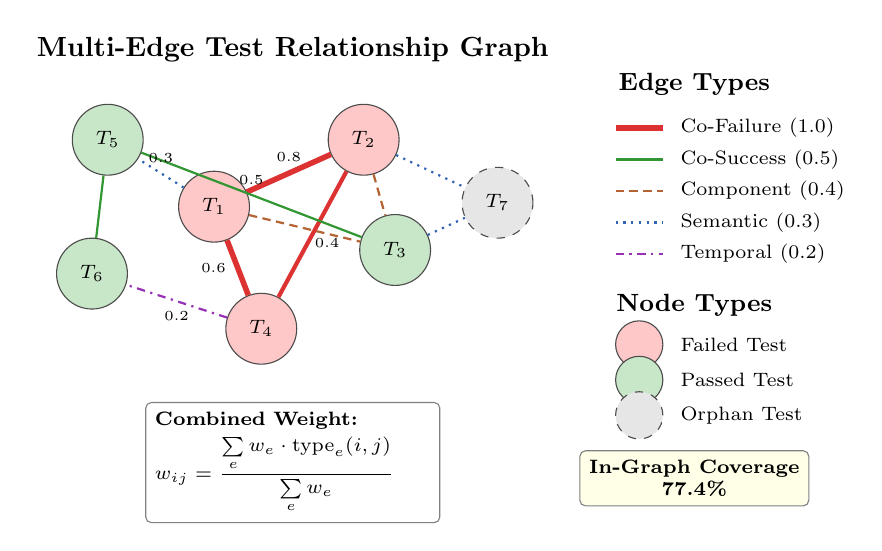
\begin{tikzpicture}[
    node distance=1.6cm,
    >=Stealth,
    every node/.style={font=\footnotesize},
    testnode/.style={circle, draw=black!70, minimum size=0.9cm,
        font=\scriptsize\bfseries, align=center},
    passnode/.style={testnode, fill=nodepass},
    failnode/.style={testnode, fill=nodefail},
    orphannode/.style={testnode, fill=nodeorphan, dashed},
    legendbox/.style={rectangle, minimum width=0.4cm, minimum height=0.15cm},
]

% === MAIN GRAPH (Left side) ===
\node[failnode] (t1) at (0, 0) {$T_1$};
\node[failnode] (t2) at (1.9, 0.85) {$T_2$};
\node[passnode] (t3) at (2.3, -0.55) {$T_3$};
\node[failnode] (t4) at (0.6, -1.55) {$T_4$};
\node[passnode] (t5) at (-1.35, 0.85) {$T_5$};
\node[passnode] (t6) at (-1.55, -0.85) {$T_6$};
\node[orphannode] (t7) at (3.6, 0.05) {$T_7$};

% === EDGES with different types ===
% Co-Failure edges (thick red)
\draw[cofailure, very thick, line width=2pt] (t1) -- (t2)
    node[midway, above, font=\tiny, black] {0.8};
\draw[cofailure, very thick, line width=2pt] (t1) -- (t4)
    node[midway, left, font=\tiny, black] {0.6};
\draw[cofailure, thick, line width=1.5pt] (t2) -- (t4);

% Co-Success edges (green, medium)
\draw[cosuccess, thick] (t3) -- (t5)
    node[midway, above, font=\tiny, black] {0.5};
\draw[cosuccess, thick] (t5) -- (t6);

% Component edges (brown, dashed)
\draw[component, thick, densely dashed] (t1) -- (t3)
    node[midway, below right, font=\tiny, black] {0.4};
\draw[component, thick, densely dashed] (t2) -- (t3);

% Semantic edges (blue, dotted)
\draw[semantic, thick, dotted] (t1) -- (t5)
    node[midway, above, font=\tiny, black] {0.3};
\draw[semantic, thick, dotted] (t3) -- (t7);
\draw[semantic, thick, dotted] (t2) -- (t7);

% Temporal edges (purple, dash-dot)
\draw[temporal, thick, dash dot] (t4) -- (t6)
    node[midway, below, font=\tiny, black] {0.2};

% === LEGEND (Right side) ===
\node[font=\small\bfseries] at (6.1, 1.55) {Edge Types};

% Legend entries
\draw[cofailure, very thick, line width=2pt] (5.1, 1.0) -- (5.7, 1.0);
\node[right, font=\scriptsize] at (5.8, 1.0) {Co-Failure (1.0)};

\draw[cosuccess, thick] (5.1, 0.6) -- (5.7, 0.6);
\node[right, font=\scriptsize] at (5.8, 0.6) {Co-Success (0.5)};

\draw[component, thick, densely dashed] (5.1, 0.2) -- (5.7, 0.2);
\node[right, font=\scriptsize] at (5.8, 0.2) {Component (0.4)};

\draw[semantic, thick, dotted] (5.1, -0.2) -- (5.7, -0.2);
\node[right, font=\scriptsize] at (5.8, -0.2) {Semantic (0.3)};

\draw[temporal, thick, dash dot] (5.1, -0.6) -- (5.7, -0.6);
\node[right, font=\scriptsize] at (5.8, -0.6) {Temporal (0.2)};

% Node legend
\node[font=\small\bfseries] at (6.1, -1.25) {Node Types};

\node[failnode, minimum size=0.6cm] at (5.4, -1.75) {};
\node[right, font=\scriptsize] at (5.8, -1.75) {Failed Test};

\node[passnode, minimum size=0.6cm] at (5.4, -2.2) {};
\node[right, font=\scriptsize] at (5.8, -2.2) {Passed Test};

\node[orphannode, minimum size=0.6cm] at (5.4, -2.65) {};
\node[right, font=\scriptsize] at (5.8, -2.65) {Orphan Test};

% === ANNOTATIONS ===
% Edge weight formula box
\node[draw=black!50, fill=white, rounded corners=2pt, font=\scriptsize,
      text width=3.5cm, align=left] at (1, -3.25) {
    \textbf{Combined Weight:}\\[2pt]
    $w_{ij} = \dfrac{\sum\limits_{e} w_e \cdot \text{type}_e(i,j)}{\sum\limits_{e} w_e}$
};

% Coverage stat
\node[draw=black!50, fill=yellow!10, rounded corners=2pt, font=\scriptsize,
      align=center] at (6.1, -3.45) {
    \textbf{In-Graph Coverage}\\
    \textbf{77.4\%}
};

% Title
\node[font=\bfseries] at (1, 2) {Multi-Edge Test Relationship Graph};

\end{tikzpicture}
\end{document}
